\section{Datenmanagement}
Zwei Aktoren wirken auf die Datenbank ein. Einerseits der Benutzer, welcher die
Informationen abfragen kann. Andererseits der DB-Administrator, welcher die
Daten abfragen, aber auch verändern und neue hinzufügen kann. Diese
Anwenungsfälle sind in der Abbildung \ref{fig:usecase} abgebildet.

\begin{figure}[h]
  \centering
     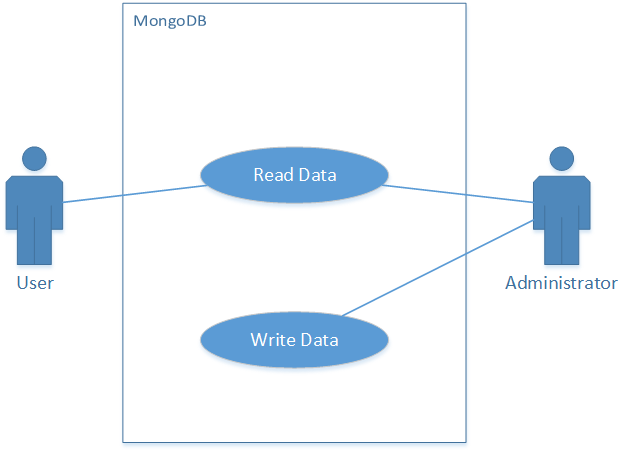
\includegraphics[width=1\textwidth]{./pictures/UseCase.png}
  \caption{Visualisierung des Anwenungsfalls}
  \label{fig:usecase}
\end{figure}

Die Daten, welche für die MongoDB verwendet werden, wurden aus der Uni-DB, welche für einige Testataufgaben im Modul DMG bereits verwendet wurde, migriert. Um diese Migration durchzuführen wurde ein Java Programm geschrieben, welches in Kapitel \ref{kap:Datenbanksprachen} näher erläutert wird. Der Strukturierte Aufbau der Datenbank wird in Kapitel \ref{kap:ERDiagramm} beschrieben.

\newpage
Der Benutzer hat die Möglichkeit, über ein GUI Daten auf der Datenbank abzufragen:
\begin{figure}[h]
	\centering
	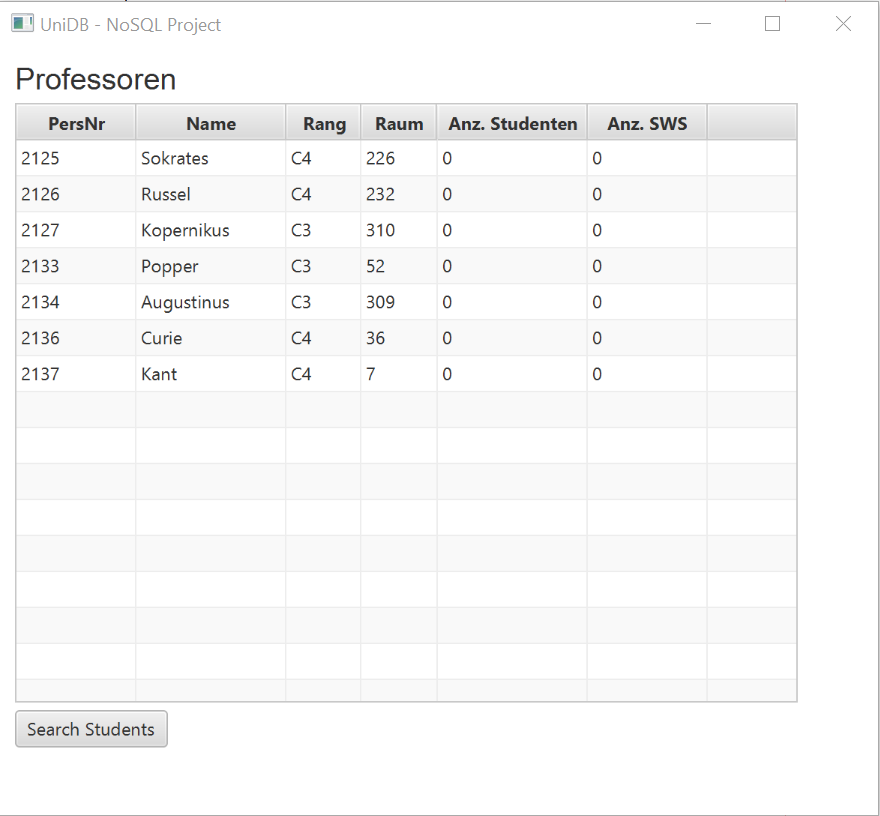
\includegraphics[width=0.5\textwidth]{./pictures/UniDBView.png}
	\caption{Gui für den Benutzer}
	\label{fig:GUI1}
\end{figure}

Über dieses GUI sind alle Professoren ersichtlich, welche in der Datenbank eingetragen sind.
Mithilfe des SearchStudents Knopf kann der Benutzer abfragen, wie viele Studenten der entsprechende Professor in seinen Vorlesungen hat, und wie viele SWS Punkte er unterrichtet.